% Environmental Research Letters (IOP Publishing, ISSN 1748-9326) submission, IOP `iopjournal` class (single-column preprint output).
% Generated by paper_erl/make_from_eris.py from paper_eris/main.tex; compile: pdflatex main && bibtex main && pdflatex main && pdflatex main
% Add the option [anonymous] to \documentclass for double-anonymous review (names, affiliations, e-mails, acknowledgments, funding, roles and data sections are then hidden).
\documentclass{iopjournal}
\usepackage{amsmath,amssymb}
\usepackage{booktabs}
\usepackage{array}
\usepackage{algorithm}
\usepackage{algpseudocode}
\setlength{\emergencystretch}{3em}
\newcommand{\dinoseg}{StrongDINOv2Seg}
\newcommand{\Lcost}{L_{\mathrm{cost}}}
\newcommand{\pending}[1]{\textcolor{red}{\textit{#1}}}% value not yet computed on the machine that generated paper_comparison_table.tex
\algrenewcommand\algorithmicrequire{\textbf{Input:}}
\algrenewcommand\algorithmicensure{\textbf{Output:}}

\begin{document}
\articletype{Letter}
\title{Smart village infrastructure planning and road network optimization for rural Telangana}
\author{Ramakrishna Kolikipogu$^{1,*}$ and Pendyala Archana$^{1}$}
\affil{$^1$Department of Information Technology, Chaitanya Bharathi Institute of Technology (A), Hyderabad, India}
\affil{$^*$Author to whom any correspondence should be addressed.}
\email{krkrishna.cse@gmail.com, pendyalaarchanareddy98@gmail.com}
\keywords{rural roads, building footprint extraction, satellite remote sensing, least-cost path, shared network, spatial transferability, open geospatial data, Telangana}
% abstract: 217 words
\begin{abstract}
Rural road planning needs to know where dwellings and public facilities are, what terrain a corridor crosses, and how neighbouring houses can share road length, yet building inventories and facility records are incomplete. We present an AI- and GIS-based pipeline from satellite imagery to shared rural access networks and apply it unchanged to four Telangana settlements: Damarakunta (rural), Adilabad (urban and fringe), Aswaraopeta (semi-urban, tribal fringe) and Alampur (heritage, semi-urban). StrongDINOv2Seg segmentation (LoveDA validation: mIoU 53.8\%, mean Dice 68.9\%) and distance-transform extraction give building footprints; a four-pass audit snaps 5, 132, 32 and 9 verified schools, colleges, hospitals, government offices and anganwadis onto roofs; a multi-criteria cost surface with a 5~m zero-crossing building clearance feeds two-stage Dijkstra routing, in which Stage~A routes each target independently and Stage~B selects a shared network by weight per marginal cost. No route crosses a building, whereas a 10~m soft footprint penalty leaves 28, 99, 157 and 5 routes across footprints. Stage~B shortened the unique network by 21.0, 12.2, 25.3 and 16.2\% (5.98, 27.12, 27.57 and 2.74~km), at an illustrative PMGSY-based cost of Rs 448, 2{,}034, 2{,}067 and 206 lakh. Segmentation footprints are unvalidated and merged roofs dominate dense fabric, so the outputs are planning alternatives that require field validation.
\end{abstract}

\section{Introduction}
Road building is among the most consequential land-use changes of the coming decades. Global road length is projected to grow by roughly 3.0--4.7 million km by 2050 \cite{meijer2018global}, and new roads open land to clearing, fragmentation and conversion \cite{laurance2014global}. Much of this growth is local. In India the Pradhan Mantri Gram Sadak Yojana (PMGSY) connects habitations through all-weather rural roads \cite{pmgsy}, and planning for such schemes depends on knowing where dwellings and facilities are, what terrain and land cover a corridor must cross, and which connection rule is applied.

Computational support for this planning has matured along three separate lines. Remote sensing now maps buildings and roads at large scale, from continental building inventories \cite{sirko2021openbuildings} to foundation-model segmenters \cite{oquab2023dinov2}, with recent work addressing small and isolated rural buildings, uncertainty, and domain shift \cite{r62,r63,r64,r65,r66,r67,r68,r69,r70}. Multi-criteria and least-cost analysis translates terrain and land cover into route costs \cite{r06,r53,r54,collischonn2000lcp}. Network-design formulations connect many demand points at low total cost, including Steiner-tree heuristics \cite{kou1981steiner,mehlhorn1988steiner,hwang1992steiner,r51}, rural road design models \cite{r41,r43,r44} and recent analogues for power and transport networks \cite{r45,r46,r47,r50}. These lines are rarely joined: detectors are judged by pixel overlap \cite{r01}, planners assume an error-free inventory, and each house is often connected independently, so neighbouring houses re-trace the same corridor.

We join them in a single reproducible pipeline and apply it, unchanged, to four settlements of different morphology in Telangana: a rural village, an urban and fringe window, a semi-urban town on a tribal fringe and a small heritage town. Our contributions are:
\begin{enumerate}
\item \textbf{End-to-end pipeline.} A pipeline from satellite imagery to a shared access network: StrongDINOv2Seg segmentation, OpenCV/NumPy distance-transform instance extraction with an explicit merge flag, a four-pass multi-source facility audit with roof snapping, a multi-criteria cost surface with a 5~m zero-crossing building clearance, and a two-stage shared-network planner (Section~\ref{sec:methods}).
\item \textbf{Error propagation.} Controlled omission and addition scenarios that propagate building-inventory errors through the planner, measuring their effect on unique length, coverage and exposure of dwellings (Sections~\ref{sec:damar}--\ref{sec:adilabad}).
\item \textbf{Four-settlement spatial transferability and open-data scalability.} The rural Damarakunta workflow is re-applied, with the same cost-surface definition and solver, to Adilabad (urban and fringe), Aswaraopeta (semi-urban, tribal fringe) and Alampur (heritage, semi-urban), end to end on Esri imagery and, for the Adilabad mandal, also on open Overture Maps footprints, with a road-gap rule for targets and robustness examined over penalty settings, road-gap thresholds and synthetic omissions (Sections~\ref{sec:adilabad} and~\ref{sec:four}).
\end{enumerate}
Two scope limits apply. Four settlements in one state were evaluated, so we make no claim about a general rural--semi-urban--urban gradient beyond them. And the segmentation results are unvalidated in every area: no reference building mask exists, and in the dense fabric of Adilabad (49\% of instances), Aswaraopeta (35\%) and Alampur (38\%) many detected instances are merged roof blocks (Sections~\ref{sec:adilabad} and~\ref{sec:four}), so their targets are built-up units rather than counted houses.

\section{Related work}
\textbf{Building extraction.} Reviews of building extraction from remote sensing \cite{r01} document the shift from fully convolutional networks \cite{ji2019whu} to transformer and foundation-model encoders. Recent studies target isolated small buildings \cite{r63}, weak supervision \cite{r62}, uncertainty-guided refinement \cite{r64,r65}, and domain generalisation or adaptation across imagery sources \cite{r02,r66,r67,r68,r69,r70}. Road extraction has followed the same path, with width-adaptive, topology-preserving and foundation-model-based networks for rural and arid scenes \cite{r56,r57,r58,r59,r60}, and topological analysis has been used to detect informal settlements worldwide \cite{r48}. Evaluation is overwhelmingly through overlap scores on benchmark data \cite{foody2002status}; the effect of detection errors on downstream infrastructure decisions is rarely quantified, although error propagation in GIS models is long established \cite{heuvelink1998error}.

\textbf{Route and network planning.} Multi-criteria GIS analysis \cite{r06} and least-cost path methods \cite{collischonn2000lcp,r53,r54} underlie corridor selection for roads, with dedicated treatments of slope \cite{r54}, route alternatives \cite{r53} and travel-time uncertainty \cite{r61}, and GIS route reconstruction has been applied to historical transport routes \cite{r55}. Rural road design has been addressed with improved network-design models \cite{r41}, algorithmic planning under constrained capacities in India \cite{r43} and facility-based methodology \cite{r44}. Steiner-tree formulations \cite{hwang1992steiner} and their shortest-path-based heuristics \cite{kou1981steiner,mehlhorn1988steiner} connect many terminals at low total length and are applied to sub-network identification \cite{r51}, multi-terminal routing \cite{r52}, cable routing \cite{r45}, minimum spanning trees of road networks \cite{r46}, rural grids \cite{r47} and least-cost electrification \cite{r50}.

\textbf{Gap.} To our knowledge no cited work combines (i) satellite-derived building instances, (ii) a land-cover- and slope-based cost surface with building avoidance, (iii) a shared-network planner whose marginal cost credits built corridors, and (iv) a systematic test of how inventory omissions and the settlement setting change the result. This paper addresses that combination for rural Telangana and treats the comparison between four settlements as an explicit transferability test.

\section{Study areas and data}
Four settlements are studied (figure~\ref{fig:flow}; table~\ref{tab:four}): Damarakunta, a rural village in Siddipet district (18.47~km$^2$); Adilabad, an urban and fringe window in Adilabad district (18.59~km$^2$); Aswaraopeta, a semi-urban town on a tribal fringe in Bhadradri Kothagudem district (2.82~km$^2$); and Alampur, a heritage and semi-urban town on the Tungabhadra in Jogulamba Gadwal district (1.65~km$^2$). All use UTM zone 44N (EPSG:32644), a 0.6~m Esri World Imagery mosaic, ESA WorldCover v200, the Copernicus GLO-30 DEM and a road layer (TGRAC for Damarakunta, Overture / OSM for the others), with 51.7, 509.9, 28.6 and 25.3~km of road inside the windows and mean terrain slopes of 3.8, 3.1, 3.1 and 2.1\%. The boundaries of Adilabad, Aswaraopeta and Alampur are derived built-up extents, not administrative boundaries.

\subsection{Damarakunta (rural)}
Damarakunta is a rural revenue village in Markook mandal, Siddipet district, Telangana ($\approx 17.707^{\circ}$N, $78.753^{\circ}$E). Its boundary, from the Telangana State Remote Sensing Application Centre (TGRAC), encloses 18.47~km$^2$ (UTM zone 44N, EPSG:32644). Settlement is dispersed, with small house clusters separated by farmland. A 0.6~m, three-band mosaic (11{,}296 $\times$ 7{,}171 px) was assembled from Esri World Imagery exports. Building candidates are model outputs: 278 polygons, 165 inside the boundary, of which 163 are used as routing targets. They carry a quality class: \textsc{Plausible} (71), \textsc{Review} (32) and \textsc{Unresolved\_Merge} (62), the last denoting blobs that merge adjacent roofs and could not be split. The facility audit (section~\ref{sec:methods}) retains five verified facilities (two schools, one health sub-centre and two gram-panchayat offices); the TGRAC anganwadi layer gives its records one shared village coordinate and was rejected as a placeholder. No ground-truth building mask exists for Damarakunta.

\subsection{Adilabad (urban and fringe)}\label{sec:adilabad_data}
Adilabad is studied in two windows. The robustness experiments of section~\ref{sec:adilabad} use the Adilabad Urban mandal polygon (geoBoundaries ADM3, 2018 release). The four-area comparison of section~\ref{sec:four} uses the updated settlement extent of Adilabad town: a built-up extent derived from ESA WorldCover (class 50) around the OpenStreetMap place node ($19.676^{\circ}$N, $78.534^{\circ}$E), 18.59~km$^2$, which covers the urban area of the Adilabad Urban mandal (50.5\%) and the adjoining built-up parts of Mavala (32.2\%) and Adilabad Rural (17.4\%). It is not an administrative boundary; an edge-continuity check found 1.5\% of the local built-up extent outside it. In this window \dinoseg{} yields 5{,}653 instances (\textsc{Plausible} 2{,}526, \textsc{Review} 181, \textsc{Unresolved\_Merge} 2{,}773, smaller than 30~m$^2$ 173), of which 613 lie more than 30~m from a road and form the targets; the road layer holds 509.9~km and the audit retains 132 verified facilities (39 schools, 15 colleges, 59 hospitals and health centres, 15 government offices, 4 anganwadis).
The 2018 window is the Adilabad Urban mandal, Adilabad district (geoBoundaries ADM3 polygon; centroid $19.682^{\circ}$N, $78.528^{\circ}$E), 17.75~km$^2$, close to Damarakunta in area. The 10~m grid has 424 $\times$ 564 cells, 177{,}533 of them inside the polygon, 0.62\% blocked (water or slope $>25^{\circ}$). About 60\% of cells are not WorldCover built-up, so the window holds an urban core and a peri-urban fringe. The boundary layer is the 2018 release and may differ from current municipal limits.

Two sets of building footprints are used. (i)~\emph{Segmentation footprints (primary, end to end).} A 0.6~m Esri World Imagery mosaic of the window (7{,}248 $\times$ 9{,}590~px, EPSG:32644) was exported with the Damarakunta recipe (1{,}800~m tiles). \dinoseg{} was applied to 391 tiles of $560\times560$~px (stride 420~px, margin 70~px, the Damarakunta tiling; Damarakunta: 459 tiles) and the same instance extraction. This yields 2{,}769 instances, of which 2{,}690 have an area of at least 30~m$^2$ and form the penalty layer; their quality classes are \textsc{Plausible} (1{,}033), \textsc{Review} (77) and \textsc{Unresolved\_Merge} (1{,}580), the last with a median area of 1{,}125.5~m$^2$ (\textsc{Plausible}: 207.4~m$^2$). Of 83 Overture place candidates inside the window, 68 are verified with the Damarakunta rule (a detected footprint within 20~m): 44 schools, 20 health and 4 government. (ii)~\emph{Open footprints (independent check).} Overture release 2026-10-21.0 \cite{overture2026} supplies 4{,}850 road segments, 24{,}924 building polygons (18{,}846 from OpenStreetMap, 6{,}078 from Google Open Buildings v3 \cite{sirko2021openbuildings}) and 738 places; footprints with area $\ge 30$~m$^2$ and confidence $\ge 0.7$ (18{,}242 polygons) form the penalty layer, and 71 of the 83 facility candidates are verified (44 schools, 20 health, 7 government) after manual removal of mis-geocoded records. Roads are Overture/OSM segments in both variants (table~\ref{tab:data}). Neither footprint set has been field-verified. Figure~\ref{fig:flow} shows the study window, the detected footprints and the verified facilities of every study area.

\begin{table}[t]
\caption{Input data and licence status. ``Not re-verified'' marks Overture licences taken from the provider documentation, which could not be opened from the execution environment.}
\label{tab:data}
\centering
\footnotesize
\begin{tabular}{@{}>{\raggedright\arraybackslash}p{3.0cm}>{\raggedright\arraybackslash}p{5.9cm}>{\raggedright\arraybackslash}p{5.5cm}@{}}
\toprule
Layer & Damarakunta / Adilabad source & Licence status \\
\midrule
Boundary & TGRAC polygon / geoBoundaries ADM3 \cite{runfola2020geoboundaries} & TGRAC: not stated / ODbL 1.0 \\
Roads, facilities & TGRAC (43 road features, 5 facilities) / Overture Maps 2026-10-21.0 \cite{overture2026} & TGRAC: not stated / ODbL 1.0 (roads), CDLA-Permissive-2.0 (places); not re-verified \\
Buildings & StrongDINOv2Seg instances (0.6~m Esri imagery; all four areas) / Overture footprints (Adilabad mandal check; OSM, Google Open Buildings v3 \cite{sirko2021openbuildings}) & Esri academic-use terms, tiles not redistributed / ODbL 1.0 and CC BY 4.0; not re-verified \\
Land cover & ESA WorldCover v200, 10~m \cite{zanaga2021worldcover} & CC BY 4.0 \\
Terrain & $\sim$30~m DEM (source not recorded) / Copernicus GLO-30 \cite{esa2022copdem}; Sobel slope, bilinear to 10~m & Not stated / Copernicus Open Access Licence \\
Training benchmark & LoveDA \cite{wang2021loveda} & Source domain only \\
\bottomrule
\end{tabular}
\end{table}

\subsection{Aswaraopeta (semi-urban, tribal fringe)}
Aswaraopeta (Ashwaraopet) is the headquarters town of Aswaraopeta mandal, Bhadradri Kothagudem district ($17.241^{\circ}$N, $81.128^{\circ}$E), on a tribal fringe. No village or town polygon exists for it in OpenStreetMap or Overture, so the study area is the built-up settlement extent derived from ESA WorldCover (class 50) around the Overture locality point, 2.82~km$^2$ and wholly inside the 2018 Aswaraopeta mandal; 8.4\% of the local built-up extent lies outside it (edge-continuity verdict clean). The mapped road layer holds 28.6~km, and 52\% of the footprints are more than 30~m from a mapped road, so the road-gap rule selects many targets. \dinoseg{} yields 1{,}297 instances (\textsc{Plausible} 772, \textsc{Review} 18, \textsc{Unresolved\_Merge} 452, smaller than 30~m$^2$ 55), 678 road-gap targets (632 routed on the clearance grid), and the audit retains 32 verified facilities: 5 schools, 3 colleges, 7 hospitals and health centres, 3 government offices and 14 anganwadis.

\subsection{Alampur (heritage, semi-urban)}
Alampur is a small heritage town on the Tungabhadra in Alampur mandal, Jogulamba Gadwal district ($15.880^{\circ}$N, $78.135^{\circ}$E), known for its temple complex. OpenStreetMap maps it only as a point, so the study area is the settlement extent derived from Overture building footprints around that node (WorldCover gave only thin slivers), 1.65~km$^2$, with 9.1\% of the local built-up extent outside it (verdict clean); it lies wholly in the Alampur mandal. The road layer holds 25.3~km. \dinoseg{} yields 430 instances (\textsc{Plausible} 208, \textsc{Review} 26, \textsc{Unresolved\_Merge} 163, smaller than 30~m$^2$ 33), 59 road-gap targets (58 routed), and the audit retains 9 verified facilities (1 school, 1 college, 2 hospitals and health centres, 5 anganwadis; no government office inside the polygon), several of them absent from Overture Places.

\section{Methods}\label{sec:methods}
The framework is a seven-step chain (figure~\ref{fig:arch}): (1)~multi-source open-data ingestion (Esri World Imagery, ESA WorldCover, Copernicus GLO-30, Overture / OSM / TGRAC roads, the study polygon); (2)~\dinoseg{} semantic segmentation in 560~px tiles; (3)~distance-transform extraction of building footprints and road-gap targets; (4)~a four-pass multi-source facility audit that snaps every facility onto a roof; (5)~a multi-criteria cost surface with a 5~m zero-crossing building clearance; (6)~Stage~A and Stage~B Dijkstra shared-network routing; and (7)~connectivity and PMGSY-based cost evaluation. Steps 1 to 7 are identical for all four study areas; the settlements differ only in their inputs. The ten-metre soft-penalty planner of the earlier experiments is kept as a comparison baseline (section~\ref{sec:damar}), and the clearance network is the proposed plan (section~\ref{sec:four}).

\begin{figure}[t]
\centering
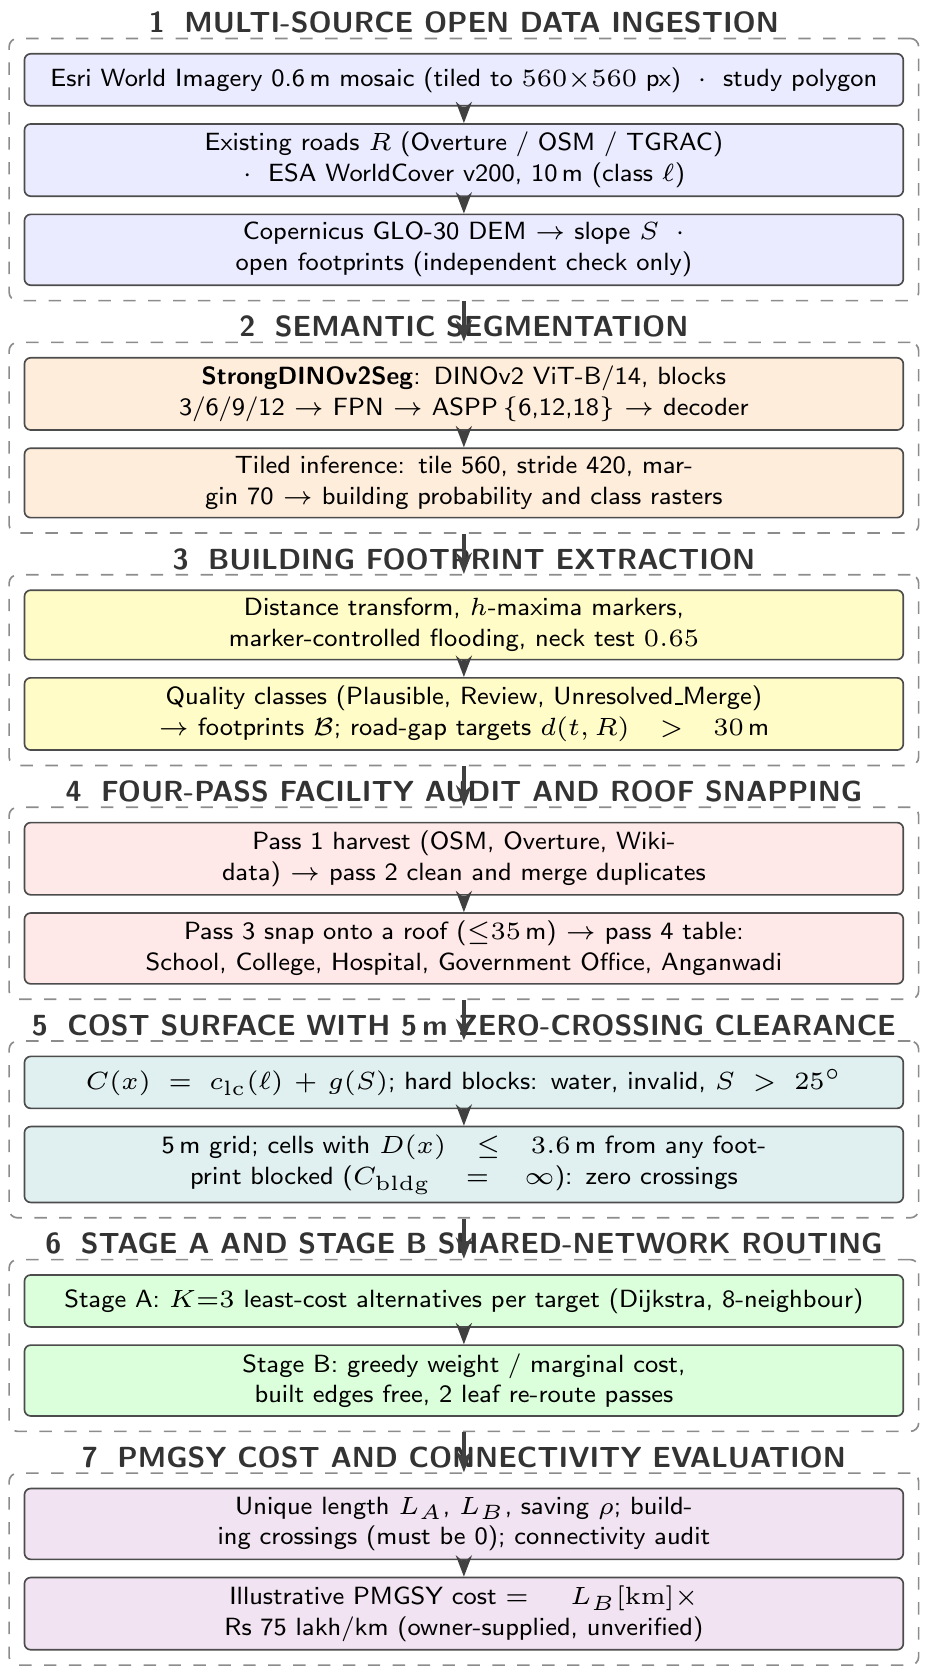
\includegraphics[width=0.5\textwidth]{fig_architecture.png}
\caption{Seven-step architecture: (1)~multi-source open-data ingestion, (2)~\dinoseg{} semantic segmentation (tile 560, stride 420, margin 70), (3)~distance-transform building footprint extraction (neck ratio 0.65), (4)~four-pass multi-source facility audit and roof snapping (School, College, Hospital, Government Office, Anganwadi), (5)~cost surface with a 5~m zero-crossing clearance (3.6~m), (6)~Stage~A independent and Stage~B shared-network Dijkstra routing, (7)~PMGSY cost and connectivity evaluation.}
\label{fig:arch}
\end{figure}

\subsection{Building extraction}
\dinoseg{} is a fully fine-tuned DINOv2 ViT-B/14 encoder \cite{oquab2023dinov2}. Tokens from blocks 3, 6, 9 and 12 are projected to 256 channels, fused (FPN-style \cite{lin2017fpn}), passed through an ASPP neck (rates 6, 12, 18) \cite{chen2018deeplabv3plus} and a four-stage decoder with auxiliary heads for deep supervision \cite{lee2015dsn}. Training used LoveDA \cite{wang2021loveda} at 560~px for a scheduled 10 epochs (AdamW, cosine schedule to $10^{-7}$, encoder learning rate $\times 0.1$) with loss $0.5\,\mathrm{CE}+0.4\,\mathrm{Dice}+0.1\,\mathrm{edge}$ \cite{milletari2016vnet} and auxiliary weight 0.4. The epoch-4 checkpoint was used; the file used for the Adilabad run has SHA-256 \texttt{2e7c4646dc77ceb2\allowbreak a357f44f11cb3f7f\allowbreak f84e636871d70ba4\allowbreak c31e194e5ec00cf3}. Building instances are extracted from the predicted mask with OpenCV and NumPy: h-maxima of the distance transform give markers, a neck test (ratio 0.65) decides whether touching blobs are split, and blobs that cannot be split are flagged \textsc{Unresolved\_Merge}.

\subsection{Road-gap targets and the open-footprint check}
For Adilabad, Aswaraopeta and Alampur the same imagery-to-footprint chain is run on Esri imagery (Section~\ref{sec:adilabad_data}), and for the Adilabad mandal Overture footprints serve as an independent check. Because connecting every footprint is meaningless in a built-up fabric already served by roads, only houses more than 30~m (the planner snap distance) from an existing road are routed. Planner cost grows roughly quadratically with the number of targets, which further motivates the filter; the threshold is varied (20, 30, 50~m) in Section~\ref{sec:adilabad}.

\subsection{Cost surface}
Let $\mathcal{B}$ be blocked cells (water, invalid cells, slope $>25^{\circ}$) and $\mathcal{P}$ the cells whose centre lies inside a footprint. The graph has the unblocked 10~m cells as nodes and 8-neighbour edges with no diagonal corner-cutting. The cell cost is
\begin{equation}
c(x)=\bigl[c_{\mathrm{lc}}(\ell(x))+g(s(x))\bigr]\,m(x),\qquad m(x)=\begin{cases}\mu & x\in\mathcal{P}\\ 1 & \text{otherwise,}\end{cases}
\label{eq:cell}
\end{equation}
where $\ell$ is the WorldCover class with resistance $c_{\mathrm{lc}}=8,5,3,6,2,4$ for trees, shrubland, grassland, cropland, built-up and bare/sparse land respectively (classes 10--60 in the order 10, 20, 30, 40, 50, 60), $g(s)=4\,\mathrm{clip}(s,0,10)/10$ with $s$ the slope in degrees, and $\mu=4$ is the footprint penalty. Edge weights are the mean end-cell cost times step length. Costs are ordinal planning units, not currency. In Damarakunta the penalty is lifted within a 20~m disc around the health sub-centre,  The land-cover, slope, cost and blocked-cell rasters are the inputs of the cost surface of every study area (figure~\ref{fig:flow}).whose point lies on the edge of its own footprint.

\subsection{Shared-network planner}
For each target, Stage~A computes a least-cost path to the existing road cells with Dijkstra's algorithm \cite{dijkstra1959note,hart1968astar,collischonn2000lcp} and alternatives by inflating costs along earlier paths ($K=3$ alternatives in total). Stage~B greedily selects the (target, alternative) pair with the highest weight per marginal cost
\begin{equation}
\Delta\Lcost\bigl(\pi\mid S\bigr)=\sum_{e\in\pi\setminus E_S}w(e),
\label{eq:marginal}
\end{equation}
where $E_S$ is the set of already selected edges, so built edges are free and a route may end on another route. This is the shortest-path heuristic for Steiner trees \cite{kou1981steiner,mehlhorn1988steiner} on a penalised, land-cover-weighted graph with the road network as a free sub-tree; it carries no optimality guarantee. Two passes of leaf re-routing follow. Snap distance is 30~m, search limit 1{,}500~m and attachment tolerance 15~m. Facilities are planned in a separate phase.

\subsection{Facility audit and roof snapping}
Overture Places alone mislocated or missed colleges, hospitals, offices and anganwadis, so the facilities of each area come from a four-pass audit (\texttt{scripts/audit\_facilities.py}). Pass~1 harvests candidates inside and within 500~m of the polygon from OpenStreetMap (Overpass and the Photon geocoder), Overture Places, Wikidata and Wikipedia (and, for Damarakunta, the TGRAC layers); LGD, UDISE+ and the district directories have no open query interface and were not used. Pass~2 assigns one of five categories (School, College, Hospital, Government Office, Anganwadi), removes closed or commercial records (pharmacies, laboratories, coaching centres, banks, cooperative societies), religious sites, foreign place names, placeholder coordinates shared by several differently named records, and merges duplicates of one campus across sources; every removal is logged with its reason. Pass~3 moves each survivor onto the footprint that contains it or, failing that, the nearest footprint of at least 25~m$^2$ within 35~m (a compound building up to 25~m away for a school, college or hospital), and removes facilities with no building in range. Pass~4 writes the verified table with the sources, the snap distance and a confidence label; records with a single source and a snap of more than 12~m are kept with \texttt{use\_in\_analysis}${}=$\,False and are not routed.

\subsection{Zero-crossing building clearance}
The soft footprint penalty $\mu$ in equation~\ref{eq:cell} lets a route cross a roof when the detour costs more. The proposed plan therefore uses a hard barrier on a finer grid. Each 10~m cost cell is refined to $2\times2$ cells of cell size $\Delta=5$~m with the same cost per metre, and every cell whose centre lies within $r_c=3.6$~m of any footprint is blocked (equation~\ref{eq:bldg}). Because $r_c>\Delta\sqrt2/2=3.54$~m, no step between two free cell centres can touch a footprint: a point of the step lies within $\Delta\sqrt2/2$ of one of its end points, and that end point would then have been blocked. A target sits inside its own building, so each route starts at the edge of that building and reaches the nearest free cell that is connected to the road network by a straight lane of at most the snap distance that touches no other footprint; a target with no such lane (a house enclosed by other buildings) is reported as unrouted, never routed over a roof. Lengths are measured from the building edge. Every drawn route (lane, path and attachment to a road) is finally intersected with all footprints other than its own.

\subsection{Mathematical formulation}
\paragraph{Segmentation loss.} With logits $\mathbf z$, labels $y$, class probabilities $p_{ic}$ and one-hot targets $t_{ic}$ at pixel $i$ (class 0 is ignored),
\begin{equation}
\mathcal L(\mathbf z,y)=0.5\,\mathcal L_{\mathrm{CE}}+0.4\,\mathcal L_{\mathrm{Dice}}+0.1\,\mathcal L_{\mathrm{edge}},\qquad
\mathcal L_{\mathrm{total}}=\mathcal L(\mathbf z^{\mathrm{main}},y)+0.4\sum_{j=1}^{3}\mathcal L(\mathbf z^{(j)},y),
\label{eq:loss}
\end{equation}
\begin{equation}
\mathcal L_{\mathrm{Dice}}=\frac1{|\mathcal C|}\sum_{c\in\mathcal C}\Bigl(1-\frac{2\sum_i p_{ic}t_{ic}+\varepsilon}{\sum_i p_{ic}+\sum_i t_{ic}+\varepsilon}\Bigr),\qquad
\mathcal L_{\mathrm{edge}}=\frac1{|\Omega|}\sum_{i\in\Omega}(1+4e_i)\,\mathrm{CE}_i,\quad e_i=\min\{1,\,|(K_x{*}y)_i|+|(K_y{*}y)_i|\}.
\label{eq:diceedge}
\end{equation}
Here $\mathcal C$ is the set of scored classes, $\varepsilon$ a small smoothing constant, $K_x,K_y$ the Sobel kernels, so that the edge term up-weights the cross-entropy of pixels on label boundaries by up to five; the three auxiliary heads $\mathbf z^{(j)}$ provide deep supervision.

\paragraph{Evaluation metrics.} From the confusion matrix, with $TP_c,FP_c,FN_c$ the true positives, false positives and false negatives of class $c$ and $N$ the number of labelled pixels,
\begin{equation}
\mathrm{OA}=\frac{\sum_c TP_c}{N},\quad P_c=\frac{TP_c}{TP_c+FP_c},\quad R_c=\frac{TP_c}{TP_c+FN_c},\quad F_{1,c}=\frac{2P_cR_c}{P_c+R_c}=\frac{2TP_c}{2TP_c+FP_c+FN_c},\quad \mathrm{IoU}_c=\frac{TP_c}{TP_c+FP_c+FN_c},
\label{eq:metrics}
\end{equation}
and $P$, $R$, $F_1$ (the Dice coefficient) and $\mathrm{mIoU}=|\mathcal C|^{-1}\sum_{c\in\mathcal C}\mathrm{IoU}_c$ are the macro averages over the scored classes. Because $F_{1,c}$ equals the per-class Dice score, the reported F1-score is the mean Dice.

\paragraph{Terrain.} Slope is taken from the Copernicus GLO-30 elevation $z$ with the Sobel gradient at the DEM spacing $\Delta_z=30$~m, resampled bilinearly to the planning grid:
\begin{equation}
\partial_x z\approx\frac{(K_x{*}z)}{8\Delta_z},\quad \partial_y z\approx-\frac{(K_y{*}z)}{8\Delta_z},\quad S=\arctan\sqrt{(\partial_x z)^2+(\partial_y z)^2},\quad p_S=100\tan S,
\label{eq:slope}
\end{equation}
with $S$ the slope in degrees and $p_S$ the equivalent percentage slope reported in the comparison table. The cost uses the linear ramp $g(S)=w_s\min(S,S_{\mathrm{ref}})/S_{\mathrm{ref}}$ with $w_s=4$ and $S_{\mathrm{ref}}=10^{\circ}$, and cells with $S>S_{\lim}=25^{\circ}$ are blocked; no separate IRC slope-penalty factor is applied.

\paragraph{Composite cost and clearance barrier.} With $c_{\mathrm{lc}}(\ell)$ the WorldCover resistance (equation~\ref{eq:cell}, so the land-cover weight is $w_{\mathrm{lc}}=1$) and $D(x)$ the Euclidean distance from the centre of cell $x$ to the nearest footprint (zero inside a footprint),
\begin{equation}
C(x)=c_{\mathrm{lc}}(\ell(x))+g(S(x))+C_{\mathrm{bldg}}(x),\qquad C_{\mathrm{bldg}}(x)=\begin{cases}\infty & D(x)\le r_c\\ 0 & \text{otherwise,}\end{cases}\qquad r_c=3.6\ \mathrm{m},\ \Delta=5\ \mathrm{m}.
\label{eq:bldg}
\end{equation}
The ten-metre comparison baseline instead multiplies the cost of cells whose centre lies in a footprint by $\mu=4$ (equation~\ref{eq:cell}).

\paragraph{Graph and routing objectives.} The graph has the free cells as nodes and 8-neighbour edges, a diagonal step being allowed only if both orthogonal neighbours are free. The weight of an edge $(u,v)$ is
\begin{equation}
w(u,v)=d(u,v)\,\frac{C(u)+C(v)}{2},\qquad d(u,v)=\begin{cases}\Delta&\text{cardinal step}\\ \sqrt2\,\Delta&\text{diagonal step.}\end{cases}
\label{eq:edge}
\end{equation}
Stage~A gives every target $t$ the independent least-cost path $\pi_t^{A}=\arg\min_{\pi:\,t\to R}\sum_{e\in\pi}w(e)$ to the existing road cells $R$ (Dijkstra), and two further alternatives that multiply $w(e)$ by $\lambda\in\{3,8\}$ on cells within $20$~m of the earlier paths and overlap them by at most 80\%. Stage~B starts from $E_S=\emptyset$ and repeatedly serves the target and route with the highest weight per marginal cost,
\begin{equation}
(t^\star,\pi^\star)=\arg\max_{t\in U,\ \pi\in\Pi_t\cup\{\pi_t^{\mathrm{net}}\}}\frac{\omega_t}{\Delta\Lcost(\pi\mid S)},\qquad
\Delta\Lcost(\pi\mid S)=\sum_{e\in\pi\setminus E_S}w(e),
\label{eq:stageb}
\end{equation}
where $U$ is the set of unserved targets, $\Pi_t$ the Stage~A alternatives, $\pi_t^{\mathrm{net}}$ the least-cost path to the roads together with the routes already selected, and $\omega_t$ the priority weight ($4$ for hospitals and health centres, $3$ for schools, colleges and anganwadis, $2$ for government offices, $1$ for houses). A built edge $e\in E_S$ thus costs nothing again, which is a discount factor $\alpha=0$ on $E_S$; no intermediate $\alpha\in(0,1)$ is used. With $L(\cdot)$ the total length of the unique edges of a route set (shared edges once),
\begin{equation}
\rho=\frac{L_A-L_B}{L_A}\times100\%,\qquad L_A=L\bigl(\{\pi_t^A\}\bigr),\quad L_B=L(E_S),\qquad X=\sum_{r}\Bigl|r\cap\bigcup_{b\ne b_r}b\Bigr|=0,
\label{eq:saving}
\end{equation}
where $X$ is the length of routes inside footprints other than the route's own building $b_r$ (zero by construction under equation~\ref{eq:bldg}).

\paragraph{Illustrative cost.} The capital cost is
\begin{equation}
\mathrm{Cost}_{\mathrm{INR\ lakh}}=L_B[\mathrm{km}]\times c_{\mathrm{PMGSY}},\qquad c_{\mathrm{PMGSY}}=75\ \text{lakh/km}\ (\text{range }60\text{--}90),
\label{eq:cost}
\end{equation}
with 1 lakh $=10^{5}$~INR. The rate was supplied by the project owner as PMGSY-based and has not been verified against a PMGSY document or a State Schedule of Rates, so the cost is illustrative and not an engineering estimate.

\subsection{Algorithms}
\begin{algorithm}[t]
\caption{Tiled \dinoseg{} inference and distance-transform building extraction (\texttt{run\_tiled\_inference.py}, \texttt{extract\_buildings\_v8.py})}
\label{alg:extract}
\begin{algorithmic}[1]
\Require mosaic $I$ (0.6~m), checkpoint $\theta$, tile $T=560$, stride $s=420$, margin $m=70$, neck ratio $\eta=0.65$, seed height $h=0.3$~m
\Ensure footprints $\mathcal B$ with quality classes
\State \textbf{assert} $s\le T-2m$ \Comment{no gaps between tile centres}
\For{each tile of size $T\times T$ at stride $s$}
  \State $p\gets\mathrm{softmax}(f_\theta(\text{tile}))$; write class $\arg\max p$ and $p_{\mathrm{bldg}}$ for the tile centre (drop $m$ px at inner edges)
\EndFor
\State $M\gets(\text{class}=\text{building})\wedge\lnot\text{no-data}$; drop components smaller than 6~m$^2$
\For{each connected component $K$ of $M$}
  \State $D\gets\mathrm{EDT}(K)$ (smoothed, $\sigma=1$ px); markers $\gets$ $h$-maxima of $D$ with height $h$
  \State pieces $\gets$ marker-controlled flooding of $-D$ (only if area $\ge 40$~m$^2$)
  \For{each adjacent piece pair $(a,b)$}
    \State $r_{ab}\gets D_{\mathrm{saddle}}/\min(D_a^{\max},D_b^{\max})$
    \If{$r_{ab}>\eta$ \textbf{or} a piece is smaller than 12~m$^2$} merge $a,b$ \Comment{no real neck}
    \EndIf
  \EndFor
\EndFor
\State polygonise; flag \textsc{Unresolved\_Merge} if area $>4\times$ the median compact roof; assign \textsc{Plausible} / \textsc{Review} / \textsc{Small} by confidence and shape
\State \Return $\mathcal B$
\end{algorithmic}
\end{algorithm}

\begin{algorithm}[t]
\caption{Cost surface with zero-crossing clearance and two-stage routing (\texttt{clearance.py}, \texttt{plan\_network\_v2.py})}
\label{alg:route}
\begin{algorithmic}[1]
\Require land cover $\ell$, DEM $z$, roads $R$, footprints $\mathcal B$, targets $\mathcal T$ (road-gap houses and verified facilities with weights $\omega_t$), $\Delta=5$~m, $r_c=3.6$~m, $K=3$
\Ensure route sets $\{\pi_t^A\}$, $E_S$ and lengths $L_A$, $L_B$, saving $\rho$, cost
\State $S\gets$ slope of $z$ (equation~\ref{eq:slope}); $C_0(x)\gets c_{\mathrm{lc}}(\ell(x))+g(S(x))$; block water, invalid cells and $S>25^{\circ}$
\State refine $C_0$ from 10~m to $\Delta=5$~m (same cost per metre); $D\gets\mathrm{EDT}(\mathcal B)$; $C(x)\gets\infty$ where $D(x)\le r_c$
\State keep the free cells connected to a road cell; edge weights $w$ by equation~\ref{eq:edge}
\For{each target $t\in\mathcal T$}
  \State entrance $e_t\gets$ point of the target's building edge nearest to a free cell $s_t$; require a lane $e_t\to s_t$ of at most 30~m that touches no other footprint, else mark $t$ unrouted
  \State $\Pi_t\gets K$ Dijkstra alternatives from $s_t$ to $R$ (corridor inflation $\lambda\in\{3,8\}$, 20~m, overlap $\le 80\%$); $\pi_t^A\gets$ first alternative
\EndFor
\State $L_A\gets L(\{\pi_t^A\})$; $U\gets$ routed targets; $E_S\gets\emptyset$
\While{$U\ne\emptyset$}
  \For{each $t\in U$} add the least-cost path $\pi_t^{\mathrm{net}}$ to $R\cup E_S$ to the candidates $\Pi_t$ \EndFor
  \State $(t^\star,\pi^\star)\gets\arg\max\ \omega_t/\Delta\Lcost(\pi\mid S)$ (equation~\ref{eq:stageb}); $E_S\gets E_S\cup\pi^\star$; $U\gets U\setminus\{t^\star\}$
\EndWhile
\State two leaf re-route passes: replace a route that no other route uses if it has become cheaper given the others
\State verify $X=0$ (equation~\ref{eq:saving}); $L_B\gets L(E_S)$; $\rho\gets 100(L_A-L_B)/L_A$; cost by equation~\ref{eq:cost}
\end{algorithmic}
\end{algorithm}

\subsection{Baselines, scenarios and metrics}
Four baselines are compared: straight lines, independent least-cost routes, a length-only control (cost surface replaced by distance) and a roads-only shared reference (routes may share edges only with the existing road network). The saving against independent routing is $\rho=(L_{\mathrm{ind}}-L)/L_{\mathrm{ind}}$, with $L$ the unique network length (shared edges counted once). The exposure metrics are the number of routes crossing another house's footprint and the route length inside other footprints. The footprint penalty is varied ($\mu\in\{1,4,20,100\}$, with a variant in which footprints are buffered by 7.1~m). For omissions, a target set $M$ is removed from the targets and from the penalty layer (a missed detection is absent from both), and the planner is re-run; random draws use seeds 1--5. Coverage, unserved households, change in unique length and length per routed target are reported.

\section{Results: Damarakunta}\label{sec:damar}
\subsection{Detection}
On the 1{,}669-image LoveDA validation split (560~px, seven scored classes) the epoch-4 checkpoint reached 53.8\% mIoU, 68.9\% Dice and 71.3\% pixel accuracy, with 72.4\% macro precision and 66.9\% macro recall; for the Building class IoU is 54.0\%, precision 62.1\% and recall 80.6\% (table~\ref{tab:seg}). These are source-domain figures, not accuracy on Damarakunta. Against Google Open Buildings v3 as a proxy (not ground truth), 118 of the 165 in-boundary candidates agree (71.5\%).

\begin{table}[t]
\caption{Detection evaluation. Top: LoveDA validation (source domain); precision and recall are macro-averages over the seven scored classes. Bottom: agreement of the 165 Damarakunta candidates with Open Buildings v3 (a proxy, not accuracy).}
\label{tab:seg}
\centering
\small
\begin{tabular}{@{}lrrrrr@{}}
\toprule
\multicolumn{6}{@{}l}{\textit{LoveDA validation split (\%)}}\\
 & mIoU & Dice & Pixel acc. & Precision & Recall\\
\midrule
StrongDINOv2Seg & 53.8 & 68.9 & 71.3 & 72.4 & 66.9\\
\quad Building class & 54.0 & 70.1 & --- & 62.1 & 80.6\\
\midrule
\multicolumn{6}{@{}l}{\textit{Damarakunta candidates vs.\ Open Buildings v3}}\\
Class & Candidates & Agree & Disagree & \multicolumn{2}{c}{Agreement (\%)}\\
\midrule
All & 165 & 118 & 47 & \multicolumn{2}{c}{71.5}\\
\textsc{Plausible} & 71 & 51 & 20 & \multicolumn{2}{c}{71.8}\\
\textsc{Review} & 32 & 14 & 18 & \multicolumn{2}{c}{43.8}\\
\textsc{Unresolved\_Merge} & 62 & 53 & 9 & \multicolumn{2}{c}{85.5}\\
\bottomrule
\end{tabular}
\end{table}

\subsection{Shared network and footprint penalty}
Independent least-cost routes for the 163 houses total 10{,}045~m, but because neighbouring houses re-trace the same corridors the unique built length is 6{,}753~m (table~\ref{tab:routing}). The two-stage plan reduces this to 5{,}069~m, a saving of 24.9\%; all 163 houses and five facilities are connected. The length-only control is 3.4\% \emph{longer} in unique length than independent cost-surface routing, and the roads-only shared reference saves 22.6\%, so most of the saving comes from sharing and a further 2.3 percentage points from sharing between new routes.

The penalty trades length for exposure (table~\ref{tab:routing}). With $\mu=1$ the plan is shortest (4{,}705~m) but 56 routes pass through other houses (660~m inside footprints). With $\mu=4$ it is 7.7\% longer while crossings halve to 28 routes and 209~m. Buffering footprints by 7.1~m with $\mu=20$ or 100 lowers crossings further (19 routes) at 6{,}190--6{,}238~m.

\begin{table}[t]
\caption{Damarakunta routing, 163 houses ($\mu=4$ unless stated). Total length counts every route; unique length counts shared edges once; $\rho$ is the saving in unique length against independent routes.}
\label{tab:routing}
\centering
\footnotesize
\begin{tabular}{@{}>{\raggedright\arraybackslash}p{4.3cm}rrrrr@{}}
\toprule
Strategy & Total (m) & Unique (m) & $\rho$ (\%) & Routes crossing & In footprints (m)\\
\midrule
Straight line (2 targets infeasible) & 8{,}092.3 & --- & --- & 60 & 1{,}453.2\\
Independent least-cost routes & 10{,}045.4 & 6{,}753.1 & 0.0 & 46 & 328.3\\
Length-only control & 9{,}166.3 & 6{,}979.8 & $-3.4$ & 64 & 1{,}615.8\\
Roads-only shared reference & 5{,}229.3 & 5{,}229.3 & 22.6 & 29 & 216.1\\
\textbf{Two-stage plan (proposed)} & \textbf{5{,}069.0} & \textbf{5{,}069.0} & \textbf{24.9} & \textbf{28} & \textbf{209.1}\\
\midrule
\multicolumn{6}{@{}l}{\textit{No footprint penalty ($\mu=1$)}}\\
Independent least-cost routes & 9{,}595.9 & 6{,}921.3 & 0.0 & 63 & 1{,}423.1\\
Two-stage plan & 4{,}705.5 & 4{,}705.4 & 32.0 & 56 & 660.1\\
\midrule
\multicolumn{6}{@{}l}{\textit{Buffered footprints (7.1~m), two-stage plan}}\\
Penalty $\mu=20$ & --- & 6{,}238.1 & 18.5 & 19 & 147.9\\
Penalty $\mu=100$ & --- & 6{,}190.3 & 18.9 & 19 & 144.8\\
\bottomrule
\end{tabular}
\end{table}

\subsection{Impact of building omissions}
Table~\ref{tab:omission} summarises the omission analysis against the 5{,}069~m baseline. Missing buildings make the plan \emph{shorter}: 10\% random omission (16 houses) understates length by 7.6\%, 20\% by 16.9\%, omission of the smallest quarter by 25.1\% and omission of all merged blobs by 29.4\%. At the same time $U$ households lose access: 16 and 33 for random 10\% and 20\% omission, 41 for the smallest quarter and 62 (38.0\%) for merged blobs. A planner reading only total length would therefore underfund the scheme. Random additions lengthen the plan by 8.6\% and 15.8\%. The saving $\rho$ stays within 24.9--26.6\% across omissions, so the benefit of sharing is robust to inventory error.

\begin{table}[t]
\caption{Impact of simulated omissions and additions, Damarakunta. Baseline 5{,}069.0~m, 163 routed. Random scenarios are means of five draws. $U$: households without a route; $\kappa$: coverage; $\delta_L$: change in unique length; $\bar\ell$: length per routed target; $\rho$: saving against independent routing.}
\label{tab:omission}
\centering
\small
\begin{tabular}{@{}lrrrrrrr@{}}
\toprule
Scenario & Routed & $U$ & $\kappa$ (\%) & $L$ (m) & $\delta_L$ (\%) & $\bar\ell$ (m) & $\rho$ (\%)\\
\midrule
Baseline & 163 & 0 & 100.0 & 5{,}069.0 & 0.0 & 31.1 & 24.9\\
Omit 10\% (random) & 147.0 & 16 & 90.2 & 4{,}684.4 & $-7.6$ & 31.9 & 25.1\\
Omit 20\% (random) & 130.0 & 33 & 79.8 & 4{,}211.5 & $-16.9$ & 32.4 & 24.9\\
Omit smallest 10\% & 146 & 17 & 89.6 & 4{,}648.6 & $-8.3$ & 31.8 & 24.9\\
Omit smallest 25\% & 122 & 41 & 74.8 & 3{,}798.3 & $-25.1$ & 31.1 & 25.6\\
Omit merged blobs & 101 & 62 & 62.0 & 3{,}579.0 & $-29.4$ & 35.4 & 26.6\\
\midrule
Add 10\% (random) & 177.4 & --- & --- & 5{,}502.4 & $+8.6$ & 31.0 & 25.6\\
Add 20\% (random) & 190.6 & --- & --- & 5{,}868.3 & $+15.8$ & 30.8 & 25.4\\
\bottomrule
\end{tabular}
\end{table}

\section{Results: robustness experiments in the Adilabad Urban mandal (2018 window)}\label{sec:adilabad}
\subsection{Road-gap targets and routing}
\emph{End-to-end run (\dinoseg{} footprints).} Of the 2{,}690 footprints of at least 30~m$^2$, 345 lie more than 30~m from a road and form the targets (Damarakunta: 163). The planner routes all 345. Independent least-cost routes total 23{,}312.5~m (unique 21{,}440.8~m); the two-stage plan needs 18{,}288.7~m, a saving of 14.7\% (table~\ref{tab:adilabad}; the routes are drawn in figure~\ref{fig:flow}). The roads-only shared reference saves 2.3\% and the length-only control 6.9\%, so almost all of the saving comes from sharing among new routes. Exposure: 54 of 345 routes (15.7\%) cross another footprint (398.0~m), against 28 of 163 (17\%) in Damarakunta.

These numbers must be read with the extraction quality in mind. More than half of the instances (1{,}580 of 2{,}769) are \textsc{Unresolved\_Merge} blobs with a median area of 1{,}125.5~m$^2$: in the dense fabric the segmenter merges neighbouring roofs, so the 345 targets are built-up units rather than houses, and the footprint penalty acts on merged blocks. No reference mask exists for Adilabad, so detection accuracy there is not known.

\emph{Open-footprint check.} With 874 road-gap targets (873 routed) among 18{,}242 Overture footprints (median footprint 139.6~m$^2$, median distance to the nearest road 42.3~m), independent routes total 56{,}308.0~m (unique 46{,}419.2~m) and the two-stage plan 34{,}358.8~m, a saving of 26.0\%; the roads-only reference saves 2.9\% and the length-only control 5.7\%; 332 of 873 routes (38\%) cross another footprint (2{,}041.1~m). The facility phase connects 71 verified facilities with 1{,}090.1~m of unique corridor.

Both Adilabad variants agree that sharing helps (14.7\% and 26.0\%) and that a roads-only reference does not (2.3\% and 2.9\%, against 22.6\% in Damarakunta), but they differ in the size of the saving. This is consistent with fewer, more widely spaced targets (345 against 874) offering less opportunity to share, an explanation that was not tested. The comparison is between two footprint sources, not a validation of either.

\begin{table}[t]
\caption{Cross-settlement comparison under the same cost surface and solver. ``Seg.'' = \dinoseg{} footprints on Esri imagery; ``open'' = Overture footprints. Targets are defined by different rules (all candidates in Damarakunta, road-gap houses in Adilabad).}
\label{tab:adilabad}
\centering
\footnotesize
\begin{tabular}{@{}>{\raggedright\arraybackslash}p{5.6cm}rrr@{}}
\toprule
Metric & Damarakunta & Adilabad seg. & Adilabad open\\
\midrule
Study area (km$^2$) & 18.47 & 17.75 & 17.75\\
Targets / routed & 163 / 163 & 345 / 345 & 874 / 873\\
Independent routes, unique (m) & 6{,}753.1 & 21{,}440.8 & 46{,}419.2\\
Length-only control, unique (m) & 6{,}979.8 & 19{,}961.2 & 43{,}787.2\\
Roads-only shared reference, unique (m) & 5{,}229.3 & 20{,}947.0 & 45{,}058.9\\
\textbf{Two-stage plan, unique (m)} & \textbf{5{,}069.0} & \textbf{18{,}288.7} & \textbf{34{,}358.8}\\
Saving vs.\ independent (\%) & 24.9 & 14.7 & 26.0\\
Roads-only shared saving (\%) & 22.6 & 2.3 & 2.9\\
Unique length per routed house (m) & 31.1 & 53.0 & 39.4\\
Routes crossing other footprints & 28 of 163 & 54 of 345 & 332 of 873\\
Length inside other footprints (m) & 209.1 & 398.0 & 2{,}041.1\\
$\mu=1\rightarrow4$: unique length change (\%) & $+7.7$ & $+9.2$ & $+13.3$\\
$\mu=1\rightarrow4$: routes crossing & 56 $\rightarrow$ 28 & 138 $\rightarrow$ 54 & 618 $\rightarrow$ 332\\
10\% random omission: change (\%) / unserved & $-7.6$ / 16 & $-8.8$ / 34 & $-7.6$ / 88\\
20\% random omission: change (\%) / unserved & $-16.9$ / 33 & $-18.3$ / 69 & $-15.0$ / 176\\
Smallest-25\% omission: change (\%) / unserved & $-25.1$ / 41 & $-21.2$ / 87 & $-21.2$ / 220\\
\bottomrule
\end{tabular}
\end{table}
\subsection{Robustness}
\emph{Footprint penalty.} Raising $\mu$ from 1 to 4 lengthens the unique network by 9.2\% and removes 84 crossing routes (138 to 54); $\mu=20$ and 100 give 19{,}777.0~m and 19{,}924.5~m with 49 and 48 routes crossing, and buffered footprints give 22{,}757.0~m and 23{,}475.5~m with 7 crossing each (table~\ref{tab:sens}). The saving against independent routing stays between 10.1\% and 17.7\% across all settings (open footprints: 17.8\% to 30.8\%, table~\ref{tab:sens_open}).

\emph{Road-gap threshold.} Targets defined as houses more than 20, 30 or 50~m from a road number 750, 345 and 129 and give savings of 10.6\%, 14.7\% and 18.5\% (open footprints: 2{,}190, 874 and 296 targets; 21.9\%, 26.0\% and 29.5\%). The saving therefore depends on the target definition, which should be reported with any such result.

\emph{Omissions.} Random omission of 10\% and 20\% (five seeds) changes unique length by $-8.8\%$ (range $-11.7$ to $-6.5$) and $-18.3\%$ ($-21.9$ to $-15.8$), leaving 34 and 69 targets unserved; single-run smallest-10\% and smallest-25\% omissions give $-8.0\%$ and $-21.2\%$ (35 and 87 unserved). As in Damarakunta and in the open-footprint check, missing buildings shorten the plan while stranding households, and the saving stays at 12.6--14.1\%. With open footprints the same scenarios give $-7.6\%$, $-15.0\%$, $-7.9\%$ and $-21.2\%$ and a saving of 23.8--25.2\%. Merged-blob and addition scenarios were not defined for Adilabad.

\begin{table}[t]
\caption{Adilabad sensitivity, \dinoseg{} footprints (345 targets unless stated). Top: footprint-penalty settings. Bottom: road-gap threshold.}
\label{tab:sens}
\centering
\footnotesize
\begin{tabular}{@{}lrrrrr@{}}
\toprule
Setting & Unique (m) & $\rho$ (\%) & Crossing routes & In footprints (m) & Targets\\
\midrule
Centre-in-footprint, $\mu=1$ & 16{,}740.5 & 17.7 & 138 & 1{,}479.8 & 345\\
Centre-in-footprint, $\mu=4$ & 18{,}288.7 & 14.7 & 54 & 398.0 & 345\\
Centre-in-footprint, $\mu=20$ & 19{,}777.0 & 12.5 & 49 & 356.4 & 345\\
Centre-in-footprint, $\mu=100$ & 19{,}924.5 & 12.2 & 48 & 343.2 & 345\\
Buffered 7.1~m, $\mu=20$ & 22{,}757.0 & 10.1 & 7 & 57.9 & 345\\
Buffered 7.1~m, $\mu=100$ & 23{,}475.5 & 10.6 & 7 & 55.7 & 345\\
\midrule
Gap $>20$~m & 30{,}621.7 & 10.6 & 69 & 442.8 & 750\\
Gap $>30$~m (primary) & 18{,}288.7 & 14.7 & 54 & 398.0 & 345\\
Gap $>50$~m & 9{,}155.2 & 18.5 & 28 & 251.9 & 129\\
\bottomrule
\end{tabular}
\end{table}

\begin{table}[t]
\caption{Adilabad sensitivity, open Overture footprints (874 targets, 873 routed). Top: footprint-penalty settings. Bottom: road-gap threshold.}
\label{tab:sens_open}
\centering
\footnotesize
\begin{tabular}{@{}lrrrrr@{}}
\toprule
Setting & Unique (m) & $\rho$ (\%) & Crossing routes & In footprints (m) & Targets\\
\midrule
Centre-in-footprint, $\mu=1$ & 30{,}335.7 & 30.8 & 618 & 4{,}893.0 & 874\\
Centre-in-footprint, $\mu=4$ & 34{,}358.8 & 26.0 & 332 & 2{,}041.1 & 874\\
Centre-in-footprint, $\mu=20$ & 37{,}024.1 & 22.8 & 271 & 1{,}687.4 & 874\\
Centre-in-footprint, $\mu=100$ & 37{,}513.9 & 21.7 & 275 & 1{,}744.8 & 874\\
Buffered 7.1~m, $\mu=20$ & 42{,}071.9 & 20.1 & 231 & 1{,}397.2 & 874\\
Buffered 7.1~m, $\mu=100$ & 44{,}094.6 & 17.8 & 221 & 1{,}310.5 & 874\\
\midrule
Gap $>20$~m & 65{,}204.4 & 21.9 & 815 & 4{,}543.9 & 2{,}190\\
Gap $>30$~m (primary) & 34{,}358.8 & 26.0 & 332 & 2{,}041.1 & 874\\
Gap $>50$~m & 15{,}880.9 & 29.5 & 126 & 809.9 & 296\\
\bottomrule
\end{tabular}
\end{table}

\section{Results: four study areas with zero-crossing clearance}\label{sec:four}
Figure~\ref{fig:flow} follows the chain of figure~\ref{fig:arch} for the four study areas, pairing for each the input (0.6~m Esri imagery, boundary and existing roads) with the final output (extracted buildings, verified facilities and the Stage~B shared network), next to a locator map of Telangana. Table~\ref{tab:four} collects every metric of the four areas; it is regenerated by \texttt{scripts/run\_village\_pipeline.py --compare-all}, and a red \pending{value} marks a number not yet computed on the machine that wrote the table. The Adilabad column uses the updated settlement boundary and the segmentation footprints of that boundary, so it is not the 2018 mandal experiment of the preceding section.

\emph{Damarakunta.} 163 road-gap targets (162 routed) from 165 extracted buildings; Stage~A 7.56~km, Stage~B 5.98~km (21.0\% shorter), 5 verified facilities, illustrative cost Rs 448 lakh; the 10~m soft-penalty plan leaves 28 routes (209~m) inside other footprints.

\emph{Adilabad.} 613 road-gap targets (607 routed) from 5{,}653 extracted buildings; Stage~A 30.87~km, Stage~B 27.12~km (12.2\% shorter), 132 verified facilities, illustrative cost Rs 2{,}034 lakh; the 10~m soft-penalty plan leaves 99 routes (677~m) inside other footprints.

\emph{Aswaraopeta.} 678 road-gap targets (632 routed) from 1{,}297 extracted buildings; Stage~A 36.89~km, Stage~B 27.57~km (25.3\% shorter), 32 verified facilities, illustrative cost Rs 2{,}067 lakh; the 10~m soft-penalty plan leaves 157 routes (1090~m) inside other footprints.

\emph{Alampur.} 59 road-gap targets (58 routed) from 430 extracted buildings; Stage~A 3.28~km, Stage~B 2.74~km (16.2\% shorter), 9 verified facilities, illustrative cost Rs 206 lakh; the 10~m soft-penalty plan leaves 5 routes (33~m) inside other footprints.

On the 5~m clearance grid Stage~B shortens the unique network relative to the independent Stage~A routes in every area (Damarakunta 21.0\%, Adilabad 12.2\%, Aswaraopeta 25.3\%, Alampur 16.2\%), and building crossings are zero in every area by construction, verified by intersecting every drawn route with all footprints. The saving is largest in Aswaraopeta, where many targets lie far from the sparse mapped road layer and share long trunks, and smallest in Adilabad, where targets are scattered over a large window. Targets with no free lane to the road network are reported as unrouted rather than routed over a roof, so the routed counts are below the target counts where buildings enclose a house. The segmentation rows are model-level: they are the LoveDA validation scores of the one checkpoint used for all four areas, not accuracy on any of them, for which no surveyed reference exists. Costs use the owner-supplied, unverified PMGSY-based rate of Rs 75 lakh/km and are illustrative.

\begin{figure}[p]
\centering
\IfFileExists{fig_flow_study_areas.png}{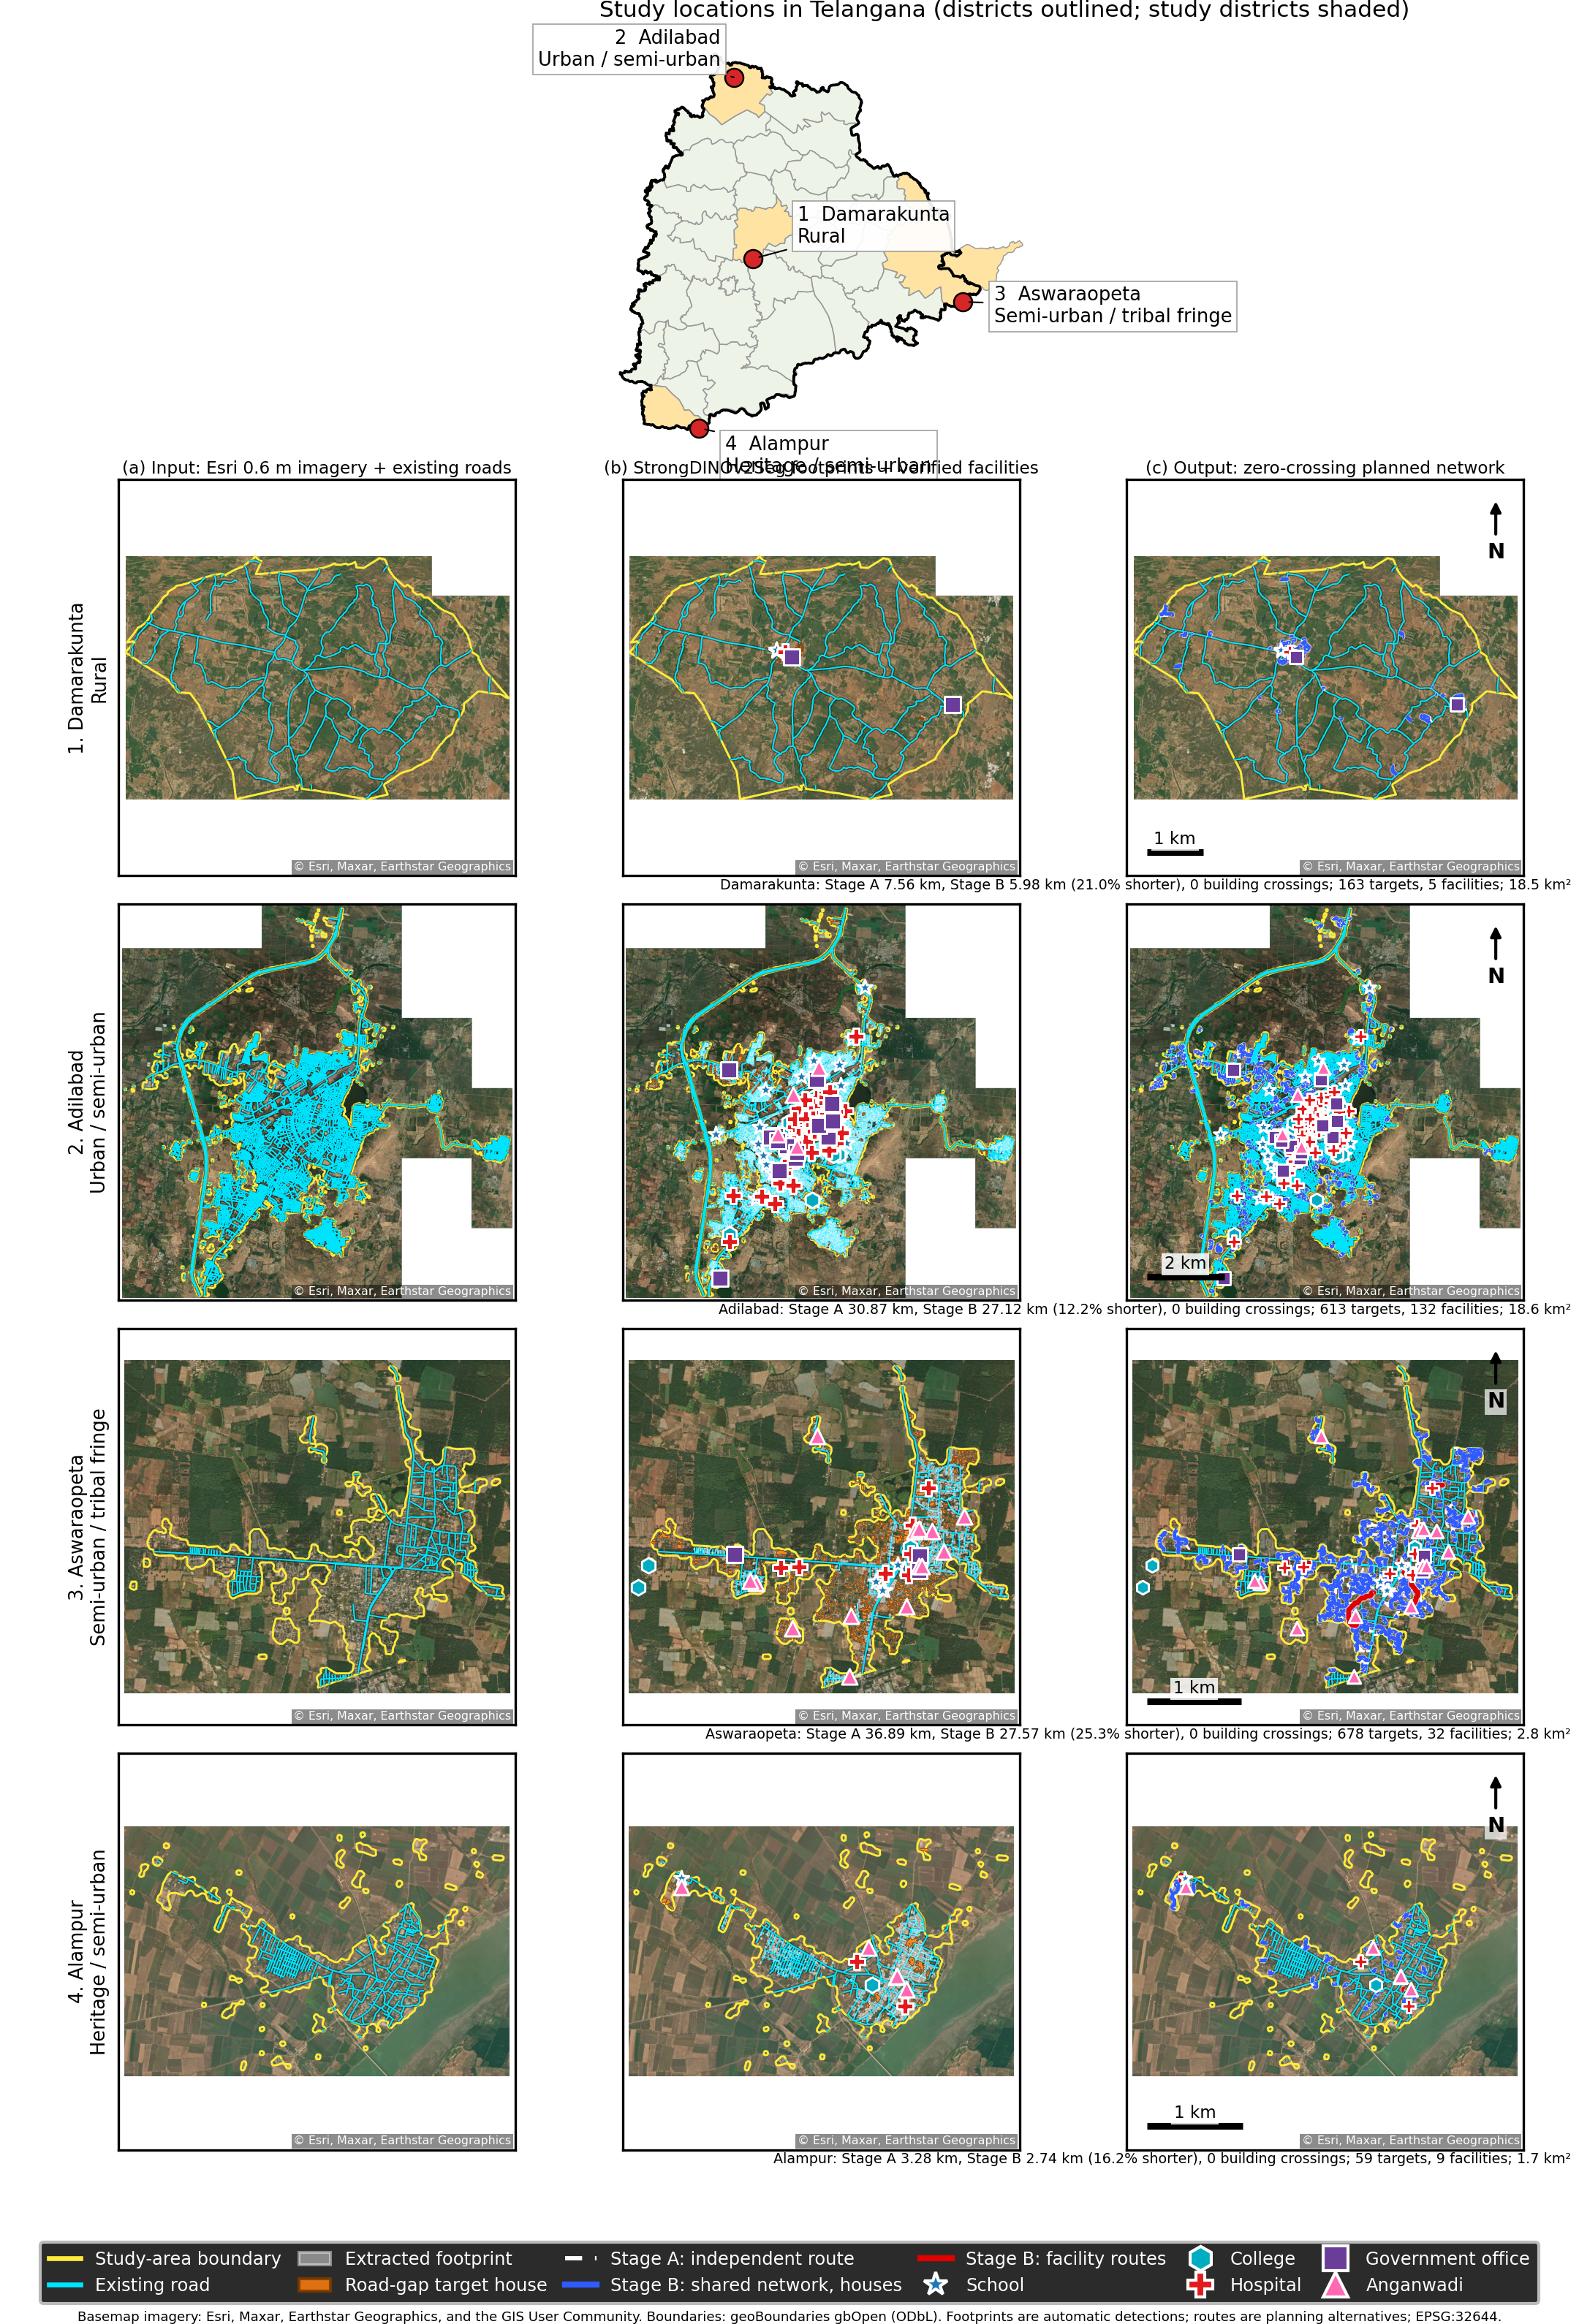
\includegraphics[width=\textwidth]{fig_flow_study_areas.png}}{\fbox{\parbox{0.8\textwidth}{\centering\pending{Figure not generated yet: run \texttt{python scripts/build\_paper\_flow\_figure.py --source segmentation} on the PC that holds the segmentation results.}}}}
\caption{Study areas and end-to-end flow. Left: Telangana with district outlines and the four study locations (1~Damarakunta, rural; 2~Adilabad, urban and fringe; 3~Aswaraopeta, semi-urban and tribal fringe; 4~Alampur, heritage and semi-urban) and the legend. Right, one strip per area in that order: input (0.6~m Esri World Imagery, study-area boundary and existing road network) $\rightarrow$ final output (the same imagery with the extracted building footprints, road-gap target houses in orange, the verified facilities---School, College, Hospital, Government Office, Anganwadi---and the Stage~B shared network of the 5~m zero-crossing plan: blue for houses, red for facilities), with scale bar and north arrow. Below each output: Stage~A and Stage~B unique length, building crossings and facility count. Basemap imagery: Esri, Maxar, Earthstar Geographics, and the GIS User Community. Footprints are automatic detections and routes are planning alternatives, not engineered roads.}
\label{fig:flow}
\end{figure}

\begin{table}[t]
\caption{Four study areas side by side. Segmentation rows: LoveDA validation of the single \dinoseg{} checkpoint (macro averages; F1-score equals the mean Dice). Routing rows: unique lengths on the 5~m zero-crossing grid (Stage~A independent, Stage~B shared network, shared edges once); building crossings are routes inside another building's footprint; the cost is the Stage~B length times Rs 75 lakh per km (range 60--90), an owner-supplied, unverified PMGSY-based rate, so it is illustrative and not an engineering estimate.}
\label{tab:four}
\centering
\scriptsize
\resizebox{\textwidth}{!}{% generated by scripts/run_village_pipeline.py --compare-all (do not edit by hand); \pending{...} marks a value not yet computed on the machine that generated this file
\begin{tabular}{@{}lrrrr@{}}
\toprule
Metric & Damarakunta & Adilabad & Aswaraopeta & Alampur \\
\midrule
\multicolumn{5}{@{}l}{\textit{Study area profile}}\\
District & Siddipet & Adilabad & Bhadradri Kothagudem & Jogulamba Gadwal \\
Typology & Rural & Urban / semi-urban & Semi-urban / tribal fringe & Heritage / semi-urban \\
Window area (km$^2$) & 0.46 & 18.59 & 2.82 & 1.65 \\
Existing road length (km) & 3.5 & 509.9 & 28.6 & 25.3 \\
\midrule
\multicolumn{5}{@{}l}{\textit{Segmentation and extraction (model metrics: LoveDA validation, one checkpoint for all areas)}}\\
Overall accuracy (\%) & \multicolumn{4}{c}{71.3} \\
Precision, macro (\%) & \multicolumn{4}{c}{72.4} \\
Recall, macro (\%) & \multicolumn{4}{c}{66.9} \\
F1-score = mean Dice (\%) & \multicolumn{4}{c}{68.9} \\
mIoU (\%) & \multicolumn{4}{c}{53.8} \\
Extracted building footprints & 100 & 5{,}653 & 1{,}297 & 430 \\
\midrule
\multicolumn{5}{@{}l}{\textit{Verified public infrastructure (audited, on building footprints)}}\\
School & 0 & 39 & 5 & 1 \\
College & 0 & 15 & 3 & 1 \\
Hospital & 1 & 59 & 7 & 2 \\
Government office & 0 & 15 & 3 & 0 \\
Anganwadi & 1 & 4 & 14 & 5 \\
Total verified facilities & 2 & 132 & 32 & 9 \\
\midrule
\multicolumn{5}{@{}l}{\textit{Stage A vs.\ Stage B routing (5\,m zero-crossing clearance) and PMGSY-benchmarked cost}}\\
Road-gap target buildings & 27 & 613 & 678 & 59 \\
Routed buildings & 27 & 607 & 632 & 58 \\
Stage A independent length (km) & 1.61 & 30.87 & 36.89 & 3.28 \\
Stage B shared-trunk length (km) & 1.31 & 27.12 & 27.57 & 2.74 \\
Corridor length saving (\%) & 18.4 & 12.2 & 25.3 & 16.2 \\
Building crossings (routes) & 0 & 0 & 0 & 0 \\
Mean terrain slope (\%) & 3.8 & 3.1 & 3.1 & 2.1 \\
PMGSY-benchmarked cost (INR lakh) & 98 & 2{,}034 & 2{,}067 & 206 \\
\bottomrule
\end{tabular}
% PMGSY-benchmarked cost = unique Stage B length (km) x Rs 75 lakh/km (sensitivity range 60-90)
}
\end{table}

\section{Discussion}
\subsection{What transfers and what does not}
The planning stages transferred without modification to all four settlements: the same cost surface, clearance rule, solver parameters and metrics produced connected plans in a dispersed village, an urban and fringe window, a semi-urban town and a small heritage town, with zero building crossings throughout. Stage~B shortened the unique network in every area (21.0\% in Damarakunta, 12.2\% in Adilabad, 25.3\% in Aswaraopeta, 16.2\% in Alampur), so sharing remains worthwhile across settlement type, though its size differs by a factor of two. In the soft-penalty experiments the qualitative findings were reproduced in Damarakunta and in the Adilabad mandal from both \dinoseg{} footprints on Esri imagery (345 targets) and open footprints (874 targets): sharing saves unique length (24.9\%, 14.7\% and 26.0\%), the footprint penalty trades length for exposure, and omissions shorten the plan while stranding households. What did not transfer is the benefit of the simpler baselines: roads-only sharing recovered most of the gain in the dispersed village (22.6\%) but almost none in the dense Adilabad window (2.3\% and 2.9\%), which suggests that the value of a marginal-cost planner grows with settlement density; Aswaraopeta and Alampur were not run with that baseline, so this remains a hypothesis supported by one dense window. The two Adilabad footprint sources differ in the size of the saving (14.7\% against 26.0\%); with merged blocks making up 57\% of the segmented instances in the mandal window, the segmentation result may reflect coarse, widely spaced targets, and no reference mask exists to say which footprint set is closer to the truth. The savings in Aswaraopeta (large) and Alampur (small window, 59 targets) also depend on how sparse the mapped road layer is, so they should not be read as a ranking of settlement types.

\subsection{Why pixel metrics are not enough for infrastructure use}
Segmentation metrics are area-weighted over classes, while the planner counts instances. A detector that misses the smallest quarter of buildings can lose few building pixels yet removes a quarter of households from the plan (table~\ref{tab:omission}), and a detector that merges adjacent roofs can score a high pixel IoU yet strands 38\% of the Damarakunta houses in the merged-blob scenario. Network length falls in both cases, so total length is a poor quality indicator. Merged blobs correspond to dense multi-roof structures; whether they coincide with the core of a hamlet was not measured.

\subsection{Land take and planning use}
Shared corridors reduce the length of new road for the same households. As an illustration only, assuming a 5~m formation width (an assumption of this study; no road-width data were available), in the soft-penalty experiments the 1{,}684~m saved in Damarakunta corresponds to about 0.84~ha less land take, the 3{,}152~m saved in the Adilabad mandal (segmentation targets) to about 1.6~ha and the 12{,}060~m saved against the open-footprint targets to about 6.0~ha; under the clearance plan the length saved by Stage~B over Stage~A corresponds to about 0.79~ha in Damarakunta (1.58~km), 1.88~ha in Adilabad (3.75~km), 4.66~ha in Aswaraopeta (9.32~km), 0.27~ha in Alampur (0.53~km). For PMGSY-style schemes \cite{pmgsy} three points follow. Building inventories are uncertain inputs and a network sized from them should carry a sensitivity band. Shared corridors save between about one eighth and one quarter of unique length and this survives omissions. Local overrides should be used sparingly and documented. The outputs are screening-level alternatives; we do not claim compliance with Indian Roads Congress design standards, nor any engineering design value.

\subsection{Limitations}
(i) Four settlements in one state; no claim is made about a general settlement gradient, and Aswaraopeta and Alampur were not run with the baselines, penalty sweeps and omission scenarios of Damarakunta and the Adilabad mandal. (ii) Omission scenarios are synthetic, not measured detection errors; merged-blob and addition scenarios were run only for Damarakunta. (iii) No area has a surveyed reference mask; the LoveDA metrics are source-domain scores of the epoch-4 checkpoint, whose metadata were recovered from the training notebook, and the checkpoint hash (SHA-256 \texttt{2e7c4646dc77ceb2\allowbreak a357f44f11cb3f7f\allowbreak f84e636871d70ba4\allowbreak c31e194e5ec00cf3}) was logged for the Adilabad run, not with the Damarakunta candidates, although both runs loaded the same file path. (iv) Merged roof blocks make up 49\% of the instances in the updated Adilabad window, 35\% in Aswaraopeta and 38\% in Alampur, so their targets are built-up units, not houses; the open footprints are map data of unverified completeness and the Overture licences were not re-verified. Ten of the 68 verified facility points of the first Adilabad run shared an identical coordinate with another Overture record (generic geocodes), so a 20~m footprint check is weak evidence in dense fabric; this is why the audit rejects placeholder coordinates. (v) The boundaries of Adilabad, Aswaraopeta and Alampur are derived built-up extents, not administrative polygons (no official polygon was available), and the Alampur extent is small (1.65~km$^2$), so its figures are noisy. (vi) The facility audit relied on OpenStreetMap, Overture Places, Wikidata and Wikipedia; LGD, UDISE+ and the district directories have no open query interface and were not used, the public Overpass servers answered only part of the queries for Damarakunta, Adilabad and Aswaraopeta (the rest came from the Photon text search), the audit snaps pins onto open Overture footprints rather than the segmentation footprints, and records with a single source and a snap of more than 12~m were excluded from the analysis; the audited counts are therefore lower bounds, not a census. (vii) Costs are ordinal, the planner is a heuristic without an optimality guarantee, the clearance plan reports targets with no free lane as unrouted, and road-gap targeting changes the problem, as the threshold sweep shows. (viii) Pixel accuracy is reported as 71.3\%, the value recomputed from the confusion matrix.

\section{Conclusions}
A pipeline from satellite imagery and open layers to shared access roads connects the houses and facilities of four Telangana settlements without changing the cost surface or solver: a rural village (Stage~B 21.0\% shorter than independent routing), an urban and fringe window (12.2\%), a semi-urban town on a tribal fringe (25.3\%) and a small heritage town (16.2\%), with a 5~m building clearance that removes every route across a roof (the 10~m soft penalty left 28, 99, 157 and 5 routes across other footprints). A four-pass multi-source audit replaced raw Overture facility points with 5, 132, 32 and 9 verified facilities of five categories snapped onto roofs. Footprint penalties and simulated inventory errors behave consistently in the soft-penalty experiments: penalties trade length for fewer routes through dwellings, and omissions shorten the plan while stranding households. The dependence of the roads-only baseline on settlement density, the effect of detection quality across settings, and the completeness of the audited facility lists are the main open questions; the Aswaraopeta and Alampur windows still need the baseline, penalty and omission experiments, and all results need field validation.

\ack{The authors acknowledge the Telangana State Remote Sensing Application Centre (TGRAC) for the boundary, road and facility layers of Damarakunta, and the providers of the open datasets used (Esri, ESA WorldCover, Copernicus DEM, Overture Maps, OpenStreetMap contributors, Wikidata, geoBoundaries, Google Open Buildings, LoveDA).}

\funding{This research received no specific grant from any funding agency in the public, commercial, or not-for-profit sectors.}

\roles{% DRAFT: the authors must confirm this statement (NISO CRediT).
Pendyala Archana: conceptualization, methodology, software, investigation, data curation, formal analysis, visualization, writing -- original draft.
Ramakrishna Kolikipogu: conceptualization, methodology, supervision, project administration, writing -- review and editing.}

\data{The data used are open and are listed with their sources:
Esri World Imagery (0.6~m tiles exported through the ArcGIS REST service, \url{https://services.arcgisonline.com/ArcGIS/rest/services/World_Imagery/MapServer}; Esri, Maxar, Earthstar Geographics, and the GIS User Community; used for non-commercial academic research under Esri's terms; the raw tiles are not redistributed);
TGRAC / BharatMaps village boundary, road and facility layers for Damarakunta (\url{https://tgrac.telangana.gov.in/}, \url{https://bharatmaps.gov.in/}; subject to the provider's terms);
Overture Maps buildings, transportation and places, release 2026-10-21.0 (\url{https://overturemaps.org/}; ODbL 1.0 and CDLA-Permissive-2.0 per theme);
OpenStreetMap through Overpass and Photon (\url{https://www.openstreetmap.org/copyright}; ODbL 1.0);
ESA WorldCover v200, 2021 (\url{https://esa-worldcover.org/}; \url{https://doi.org/10.5281/zenodo.7254221}; CC BY 4.0);
Copernicus DEM GLO-30 (\url{https://doi.org/10.5270/ESA-c5d3d65});
LoveDA (\url{https://doi.org/10.5281/zenodo.5706578});
Wikidata and Wikipedia (\url{https://www.wikidata.org/}); geoBoundaries gbOpen (\url{https://www.geoboundaries.org/}; ODbL 1.0).
Code, derived summary tables, the facility audit tables (verified facilities and every exclusion with its reason), the boundary provenance files and the open-data manifests with SHA-256 hashes are available at \url{https://github.com/Archana519/Telangana-Rural-Project} (folders \path{FINAL_PROJECT_OUTPUTS}, \path{DELIVERABLES_DAMARAKUNTA_STAGE_B} and \path{DELIVERABLES_CONTRIBUTION_3_MULTI_VILLAGE}); the source list with licences is \path{FINAL_PROJECT_OUTPUTS/00_SOURCES_AND_PROVENANCE/SOURCES_AND_PROOFS.md}. Licences were not re-verified by the authors.}

\section*{Conflict of interest}
The authors declare no competing interests.

\section*{References}
\bibliographystyle{iopart-num}
\bibliography{references}

\end{document}
